\section{Viscoelastic Material Analysis Metrics}\label{sect:ve_analysis}

The System Dependency and Phantoms Task Force identified that ``simple'',
analytic viscoelastic material models, such as Voigt and Maxwell materials,
inadequately capture the phase velocity trends measured across the energetic
frequency ranges associate with liver shear wave speed characterization [CITE].
Instead of using an analytic VE material model, we proposed characterizing the
phantoms using a linear dispersion model of the form

\begin{equation}
c(f) = c_0 + \frac{dc}{df} f.
\end{equation}

This linear model was fit to the 2D Fourier transform of axial velocity data
over a frequency range of 100--400 Hz, and two metrics were used to
characterize the viscoelasticity of materials:

\begin{enumerate}
    \item Phase velocity at 200 Hz ($c_{200}$), and
    \item Line phase velocity slope from 100--400 Hz ($\frac{dc}{df}$).
\end{enumerate}

This model was applied to human data in patients with liver
fibrosis~\cite{Palmeri2011} (Figure~\ref{fig:phantom_liver_scatter_plot}) to
establish a range of realistic linear dispersion VE material values for healthy
through advanced fibrosis liver health.

\begin{figure}[htb!]
    \centering
    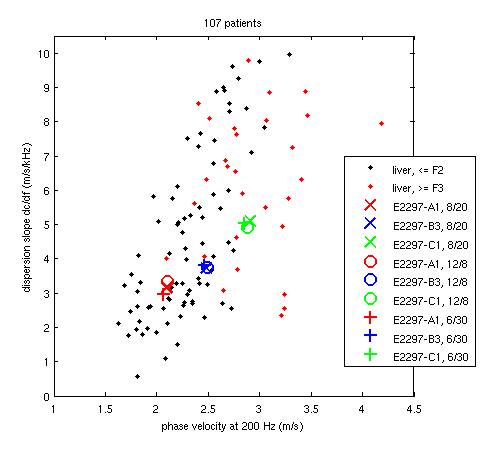
\includegraphics[width=0.75\linewidth]{phantom_liver_scatter_plot.png}
    \caption{Scatter plot comparing mechanical properties of liver (black, red
        dots) in 107 patients with measurements from the CIRS E2297-A1, B3, and
        C1 phantoms made on August 20, 2014 (X’s), December 8, 2014 (O’s), and
        June 30, 2015 (+’s). Points are plotted as a function of (200 Hz) and
        $\frac{dc}{df}$ from a linear dispersion model from 100--400 Hz.}
\label{fig:phantom_liver_scatter_plot}
\end{figure}


\begin{figure}[htb!]
    \centering
    \begin{tabular}{c}
        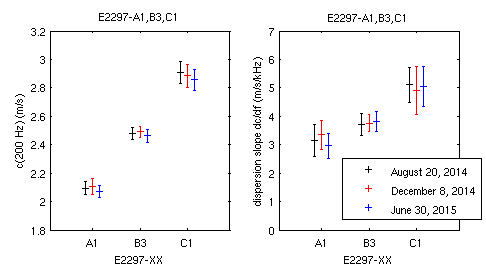
\includegraphics[width=0.75\linewidth]{figs/phase2_longitudinal_stability.png} \\
        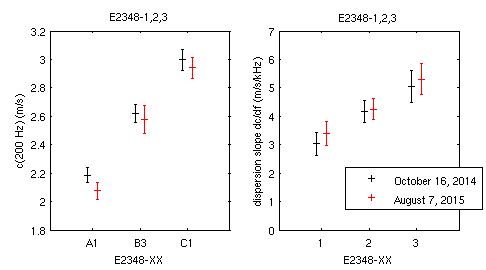
\includegraphics[width=0.75\linewidth]{figs/phaseIIset2_temporal_stability.png} \\
    \end{tabular}
    \caption{Results for the quantities $c_{200}$ (left) and dispersion slope
        $\frac{dc}{df}$ (right) for phantoms [TOP ROW] E2297-A1, B3, and C1
        from measurements made on August 20, 2014 (black), December 8, 2014
        (red), and June 30, 2015 (blue) and [BOTTOM ROW] E2348-1, -2, and -3
        from October 16, 2015 and August 07, 2015. The data points represent
        the mean $\pm$ standard deviation from 16 measurements in each
        phantom.} \label{fig:phase2_longitudinal_stability}
\end{figure}

